\documentclass{article}

\usepackage[parfill]{parskip}
\usepackage{graphicx}
\usepackage{amsmath}
\usepackage{tikz}
\usepackage[utf8]{inputenc} % For åäö

\title{"Catch and Throw" ball and beam process\\FRTN01 -- Real-Time Systems}
\author{
Mattias Fält -- faldt.mattias@gmail.com
\and
Lucas Jimbergsson -- lucas@jimbergsson.se
\and
Erik Nossborn -- eki.nossborn@gmail.com
\and
Iulia Stoica -- mariajstoica@gmail.com
}

\begin{document}
\maketitle

\section{Introduction}
% Should state the problem to be solved

\section{Process model}
\subsection{System Equations}


The equation for a ball on a beam was taken from the material from the first lab in the course, and can be written as

\begin{equation}
m(\ddot{x}-x\dot{\phi}^{2})=-mg\sin(\phi)-\frac{2}{5}m\ddot{x},
\end{equation}
where $x$ is the distance of the ball along the beam, $m$ is the mass of the ball and $\phi$ is the angle of the beam.

We chose a simple model for the beam, letting the control signal be proportional to the torque on the beam.
To account for the displacement of the beam around the rotational center, we modeled a force proportional to the angle of the beam.
This approximation turned out to be quite good, especially for small angles.
The last part of this model is the force applied to the beam by the ball.
The differential equation is given as
\begin{equation}
J_{B}\ddot{\phi}=k_{u}u+mgx\cos(\phi)+k_B\phi,
\end{equation}
where $J_{B}$ is the moment of inertia of the beam, $k_u$ is the torque to control signal ratio and $k_B$ the estimated torque per radian from the displacement of the beam.\\
\\
Letting $x_{1}=x,\, x_{2}=\dot{x},\, x_{3}=\phi,\, x_{4}=\dot{\phi}$,
we can then write the system as a set of first order nonlinear differential equations

%\begin{eqnarray*}
%m(\dot x_{2}-x_{1}x_{4}^{2}) & = & -mg\sin(x_{3})-\frac{2}{5}m\dot{x}_{2}\\
% & \Leftrightarrow\\
%\dot{x}_{2} & = & \frac{5}{7}\left(-g\sin(x_{3})+x_{1}x_{4}^{2}\right)
%\end{eqnarray*}
%
%
%and beam equation as
%\[
%\dot{x}_{4}=\frac{1}{J_B}\left(k_{u}u+mgx_{1}\cos(x_3)+k_Bx_3\right).
%\]
%
%
%We thus have then nonlinear first order system equations

\[
\begin{pmatrix}\dot{x}_{1}\\
\dot{x}_{2}\\
\dot{x}_{3}\\
\dot{x}_{4}
\end{pmatrix}=\begin{pmatrix}x_{2}\\
\frac{5}{7}\left(-g\sin(x_{3})+x_{1}x_{4}^{2}\right)\\
x_{4}\\
\frac{1}{J_B}mgx_{1}\cos(x_3)+\frac{k_B}{J_B}x_3
\end{pmatrix}+\begin{pmatrix}0\\
0\\
0\\
\frac{k_{u}}{J_B}
\end{pmatrix}u.
\]

\subsection{Linearization}

We introduced the mass of the ball as a state $x_{5}=m$ in the system. The advantage of this is that it would then be possible to start estimating the weight of the ball earlier in the sequence.
It would also allow feed forward to the control signal based on the mass and position of the ball, this could have greatly reduced the oscillations of the beam control since we would not require integral action to account for this entire force.
We lastly introduced the integral of the deviation of the position of the
ball $(\tilde{x}_{6}=\int_{0}^{t}\tilde{x}_{1}dt)$ as a state and linearized the system around the steady state $\bar{x}=(\bar{x}_{1},0,0,0,\bar{m},\bar{u})$.
This results in the linear perturbation equations
%\begin{eqnarray*}
%\dot{\tilde{x}} & = & \begin{pmatrix}0 & 1 & 0 & 0 & 0\\
%\frac{5}{7}\bar{x}_{4}^{2} & 0 & -\frac{5g}{7}\cos(\bar{x}_{3}) & 2\bar{x}_{1}\bar{x}_{4} & 0\\
%0 & 0 & 0 & 1 & 0\\
%\bar{m}\frac{g}{J_B}\cos(\bar{x}_{3}) & 0 & -\bar{m}\frac{g}{J_B}\bar{x}_{1}\sin(\bar{x}_{3})+\frac{k_B}{J_B} & 0 & \frac{g}{J_B}\bar{x}_{1}\cos(\bar{x}_{3})\\
%0 & 0 & 0 & 0 & 0
%\end{pmatrix}\tilde{x}+\begin{pmatrix}0\\
%0\\
%0\\
%\frac{k_{u}}{J_B}\\
%0
%\end{pmatrix}\tilde{u}\\
% & = & \begin{pmatrix}0 & 1 & 0 & 0 & 0\\
%0 & 0 & -\frac{5g}{7} & 0 & 0\\
%0 & 0 & 0 & 1 & 0\\
%\bar{m}\frac{g}{J_B} & 0 & \frac{k_B}{J_B} & 0 & \frac{g}{J}\bar{x}_{1}\\
%0 & 0 & 0 & 0 & 0
%\end{pmatrix}\tilde{x}+\begin{pmatrix}0\\
%0\\
%0\\
%\frac{k_{u}}{J_B}\\
%0
%\end{pmatrix}\tilde{u}.
%\end{eqnarray*}

\begin{eqnarray*}
\dot{\tilde{x}} & = & \begin{pmatrix}0 & 1 & 0 & 0 & 0 & 0\\
0 & 0 & -\frac{5g}{7} & 0 & 0 & 0\\
0 & 0 & 0 & 1 & 0 & 0\\
\bar{m}\frac{g}{J_B} & 0 & \frac{k_B}{J_B} & 0 & \frac{g}{J_B}\bar{x}_{1} & 0\\
0 & 0 & 0 & 0 & 0 & 0\\
1 & 0 & 0 & 0 & 0 & 0
\end{pmatrix}\tilde{x}+\begin{pmatrix}0\\
0\\
0\\
\frac{k_{u}}{J_B}\\
0\\
0
\end{pmatrix}\tilde{u}\\
 & = & A\tilde{x}+B\tilde{u}\\
\tilde{y} & = & \begin{pmatrix}1 & 0 & 0 & 0 & 0 & 0\\
0 & 0 & 1 & 0 & 0 & 0
\end{pmatrix}\tilde{x}+w=C\tilde{x}
\end{eqnarray*}
where $\tilde{x}=x-\bar{x}$, $\tilde{u}=u-\bar{u}$.
\\
The system is now in a form that works with the LQG framework.

%where $v$ and $w$ has intensity matrices $V$ and $W$. We now define
%the cost function $J=E\left[\int_{0}^{\infty}\tilde{x}^{T}Q\tilde{x}^{T}+u^{T}\frac{1}{r^{2}}u\, dt\right]$,
%with $Q=\text{diag}\left(\frac{1}{q_{1}^{2}},\frac{1}{q_{2}^{2}},\frac{1}{q_{3}^{2}},\frac{1}{q_{4}^{2}},\frac{1}{q_{5}^{2}}\right)$
%and let the controller be

%\begin{eqnarray*}
%\dot{\hat{x}} & = & A\hat{x}+B\tilde{u}+K(y-C\hat{x})\\
%\tilde{u} & = & -L\hat{x}.
%\end{eqnarray*}


%The optimal $K$ and $L$ is then given by the symmetric positive
%definite solutions $P$ and $S$ to 
%\begin{eqnarray*}
%0 & = & AP+PA^{T}-PC^TW^{-1}CP+V\\
%0 & = & A^{T}S+SA-SBR^{-1}B^{T}S+Q
%\end{eqnarray*}


%as $K=PC^{T}W^{-1}$ and $L=R^{-1}B^{T}S$.

%An initial guess for the matrices $Q$ and $R$ could be given by
%giving similar penalty for deviations $(3cm,1cm/s,2^{\circ},0.5^{\circ}/s,-,20cm\cdot s)$
%and $(1V)??$. Thus

%$Q=\text{diag}(1111,10000,816,13131,0,25)$, $R=1.$


\subsection{Throw Equations}

To be able to throw the ball to a desired location we needed to know how the relation between the terminal state of the ball on the beam and the distance traveled in the air.
We derived this relation using the nonlinear system equations above and the equations for a free falling body.
The resulting equations are

%\begin{eqnarray*}
%h & = & h_{0}+v_{y_{0}}t-\frac{gt^{2}}{2}\\
%d & = & d_{0}+v_{x_{0}}t,
%\end{eqnarray*}


%which results in the terminal time $t_{T}=(d_{T}-d_{0})/v_{x_{0}}$.

%We desire 
%\begin{eqnarray*}
%h_{T} & = & -d_{y}\\
%d_{T} & = & d_{x},
%\end{eqnarray*}


%and know
%\begin{eqnarray*}
%h_{0} & = & l\sin(\phi)\\
%d_{0} & = & l\cos(\phi),
%\end{eqnarray*}


%which gives
%\begin{eqnarray*}
%-d_{y} & = & l\sin(\phi)+v_{y_{0}}t-\frac{gt^{2}}{2}\\
%d_{x} & = & l\cos(\phi)+v_{x_{0}}t.
%\end{eqnarray*}


%The velocity of the ball in the horizontal and vertical directions
%are
%\begin{eqnarray*}
%v_{x} & = & \dot{x}\cos(\phi)-x\dot{\phi}\sin(\phi)\\
%v_{y} & = & \dot{x}\sin(\phi)-x\dot{\phi}\cos(\phi),
%\end{eqnarray*}


%and at the release-time, we have $x=l$. These equations gives
\begin{eqnarray*}
-d_{y}(t) & = & l\sin(\phi)+\left(\dot{x}\sin(\phi)-l\dot{\phi}\cos(\phi)\right)t-\frac{gt^{2}}{2}\\
d_{x}(t) & = & l\cos(\phi)+\left(\dot{x}\cos(\phi)-l\dot{\phi}\sin(\phi)\right)t,
\end{eqnarray*}
where $d_{y}(t), d_{x}(t)$ are the distances traveled after time $t$ as given in Figure \ref{fig:throw} and $(x=l,\dot x,\phi, \dot{\phi})$ is the state when the ball is leaving the beam.

\begin{figure}[\textwidth]
\centering
\begin{tikzpicture}[scale=1.5]
\usetikzlibrary{patterns,snakes}
\definecolor{Darkgreen}{rgb}{0,0.4,0}
\tikzstyle{brace} = [decorate, decoration={brace, amplitude=5pt}]

\node[inner sep=0] (v0) at (0,0) {};
\node[inner sep=0] (v2) at (2,0.5) {};
\node[inner sep=0] (v1) at (-1,-0.25) {};

\draw[color=red]  (v1) edge (v2);

\node (v3) at (8,-2) {};
\node (v4) at (0,-2) {};
\node (v5) at (8,0) {};

\draw[ball color=blue] (2,0.6) circle (.1);

\draw[dashed,->] (v2) -- (4,1) node[pos=1,above] {$\dot{x}$};
\draw[dashed] (v0) -- (v5) {};
\draw[dashed] (v0) -- (v4) {};
\draw[brace] (v0) -- (v2) node[pos=0.5,above,yshift=6] {$l=x$};
\draw[brace] (v3) -- (v4) node[pos=0.5,below,yshift=-6] {$d_x$};
\draw[brace] (v5) -- (v3)  node[pos=0.5,right,xshift=5] {$d_y$};

 \draw[color=green] plot[smooth] coordinates {(v2) (4,0.6) (6,0) (8,-2)};
 
 
\node at (1.3,0.17) {$\phi$};

\path[clip] (2,0.5) -- (0,0) -- (2,0);
\node[circle,draw=Darkgreen, minimum size=90pt] at (0,0) (circ) {};

\end{tikzpicture}
\caption{Illustration of the ball and its calculated trajectory as it is leaving the beam.}
\label{fig:throw}
\end{figure}
%
%and from the second equation we arrive at 
%\[
%t=\frac{\left(d_{x}-l\cos(\phi)\right)}{\dot{x}\cos(\phi)-l\dot{\phi}\sin(\phi)},
%\]
%

%and can thus insert that into the first equation:
%\begin{gather*}
%-d_{y}=l\sin(\phi)+\frac{\left(\dot{x}\sin(\phi)-l\dot{\phi}\cos(\phi)\right)\left(d_{x}-l\cos(\phi)\right)}{\dot{x}\cos(\phi)-l\dot{\phi}\sin(\phi)}-\frac{g}{2}\left(\frac{\left(d_{x}-l\cos(\phi)\right)}{\dot{x}\cos(\phi)-l\dot{\phi}\sin(\phi)}\right)^{2}.
%\end{gather*}

To be able to find a satisfactory terminal state we made the assumption of zero terminal angular velocity of the beam ($\dot{\phi}=0$). This allows us to explicitly solve for the relation between terminal ball velocity and angle of the beam as

%\subsection{Assuming $\dot{\phi}=0$}
%
%We can simplify the equation if we assume stationary beam at realease
%($\dot{\phi}=0$) 
%\begin{eqnarray*}
%-d_{y}\dot{x}^{2}\cos^{2}(\phi) & = & \dot{x}^{2}\cos^{2}(\phi)l\sin(\phi)+\dot{x}^{2}\cos(\phi)\sin(\phi)\left(d_{x}-l\cos(\phi)\right)-\frac{g}{2}\left(d_{x}-l\cos(\phi)\right)^{2}
%\end{eqnarray*}
%simplify:
%
%\[
%-d_{y}\dot{x}^{2}\cos^{2}(\phi)=\dot{x}^{2}\cos(\phi)\sin(\phi)d_{x}-\frac{g}{2}\left(d_{x}-l\cos(\phi)\right)^{2}
%\]
%
%
%and we can then finally solve for $\dot{x}$:
%
\[
\dot{x}=\left(d_{x}-l\cos(\phi)\right)\frac{\sqrt{g}}{\sqrt{2\cos(\phi)\left(d_{y}\cos(\phi)+d_{x}\sin(\phi)\right)}}.
\]

Given a fix $d_x,d_y$ it is now possible to find a pair of $\dot x,\phi$ to which we could generate a trajectory using the iterative gradient based method described in \cite{NR}, chapter 21.1.1.

One example of a generated trajectory for the process using this framework can be seen in Figure \ref{fig:matlabtrajectory}.

\begin{figure}[\textwidth]
\centering
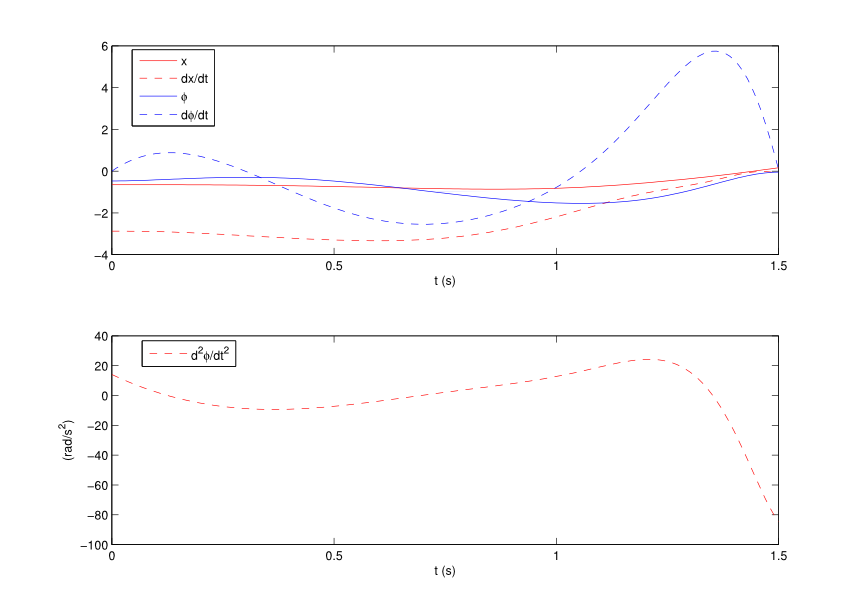
\includegraphics[width=\textwidth]{ballbeammatlab}
\caption{Example of trajectory generated using the gradient based iterative optimization. The states are plotted as deviations from the desired terminal condition. The second derivative of the angular velocity of the beam is used as control signal in this example, that that could easily be recalculated to the force required by the controller using the model.}
\label{fig:matlabtrajectory}
\end{figure}

\section{Controller structure}
% Should describe the control design aspects of the project.

\section{Program structure}
% Should describe the main program structure, both from a class and and a real-time perspective. If possible illustrate this with some type of figure.

\section{Operator communication}
% Should describe the user interface in the project including a short HowTo description on how to start and operate the program.

\section{Results}
% A section containing the results. In case the project is a control-oriented project this should include plots of measurement signals, reference signal, and control signal. If the project is more of a real-time nature then this section could contain measurement results of different type.

\section{Conclusions}


\newpage
\begin{thebibliography}{9}
\bibitem{NR}
  Thomas Bewley,
  \emph{Numerical Renaissance: simulation, optimization, \& control}.
  Renaissance Press,
  http://numerical-renaissance.com/NR.pdf

\end{thebibliography}

\end{document}



%From suggested solution:
%\section{System model}
%We will use the model from the lab in the course, but modify it to account for the extra integrator. We will then estimate the model parameters through simple experiments on the model.
%
%\section{Regulator structure}\label{regstruc}
%We are planning to use different regulator structures for the different parts of the execution. The idea is that we will use a simple PID controller to move the beam to the pick-up position and then an LQG controller for the other parts.
%\subsection{Step 1, Beam control}
%We will use a simple PID controller for the position of the beam in this part. A gradually increasing reference will be given for the beam until indication is given by the sensor, that the beam is in the pick-up position. The reference will then stay constant for some time until the ball has rolled onto the beam, and the next controller is started. The controller for this part is governed by the BeamRegul class.
%\subsection{Step 2, Ball balancing}\label{step2}
%This part will be regulated by a time-invariant LQG regulator. The model will be linearized around a desired position for weighing it. As the model will depend on the mass of the ball, there is a risk of this approach not being robust enough (for all weights of the balls). Hence, if needed we will introduce the ball weight as a state in the model, which can be estimated by the Kalman-filter. We might switch to a cascaded PID controller if this method is too hard to implement or is taking too much time.
%\subsection{Step 3, Ball delivery}
%Depending on the mass of the ball, different actions will be done. We will have the same structure for all controllers in this part, but different reference values. The idea for all of them is to first find a nominal solution of the control signal $u$ and state $\mathbf{x}$ trajectories to the nonlinear equations, and then control the system using time-varying LQG regulators. It might be beneficial to have an intermediate regulator that moves the system to a state different from the weighing state, before we execute these controllers, to get a better initial state for the optimization method described below.
%\subsubsection{Finding a solution}
%We have several ideas on how to solve this part. We can either use JModelica to find an optimal trajectory similar to what is done in Nonlinear Control Lab 3. If this requires too much time, we might also use a numerical optimization approach in MATLAB, as outlined in for example \cite{NR} chapter 21.1.1. Lastly, if these methods fail or provide unsatisfactory solutions, we could make a simple ansatz and find an analytical solution.
%\subsubsection{Calculating regulator}
%The method above would generate a trajectory $(u, \mathbf{x})$ that satisfies the specific goal for the current ball. We will then linearize the process model around the trajectory, resulting in a linear time-varying system. We can then, using MATLAB, solve the differential Riccati equation for the linearized system using some simple numerical solver. This would generate a feedback and estimation matrix for each timestep which can be saved to disk.
%\subsubsection{Executing regulator}
%Each regulator can read its respective feedback and estimation values for each time-step at initiation and will then simply apply them in real time.
%
%
%\section{Transition between controllers}
%When going from one controller to another, the control signal may very well make a jump from one value to another. The bumps introduced may be problematic if they are considerable and not dealt with. As compared to the newer ball and beam process used in Lab 1 however, our older process has an extra integrator (torque instead of angular velocity as input signal) which gives an even stronger lowpass behavior. This will indeed smooth the bumps but we will have to investigate whether, and to what extent, we have to deal with them.
%
%One idea we have for dealing with bumps, is to initially run the control signal through a lowpass filter after a switch of controller. In the initial time frame when lowpass filtering is active however, the controller will be slow, so the filter has to be deactivated before we allow the reference signal to change.
%
%\section{UML}
%
%An overview of the classes is shown in figure \ref{fig:UML}. 
%The responsibilities of each class are as follows:
%\begin{itemize}
%\item Main: the constructor creates an instance of the first controller to be run and it also creates and starts an instance of its internal thread called MainThread. This thread is the one performing the calculations of the control signal with the help of methods of the current controller.
%\item Regul: is an abstract class which all the controllers inherit from. It contains a thread whose task is to check if the work of the currently running controller is finished and it also checks if the program should switch to a different controller. It has an internal monitor called ParamMonitor which communicates with the Gui thread. The RefBeamMonitor is valid only for the controller of the beam.
%\item Measurement and OutSignal are help classes, the first containing measurement signals and the latter containing the outputs
%\end{itemize}
%
%\begin{figure}[htbp]
%  \centering
%  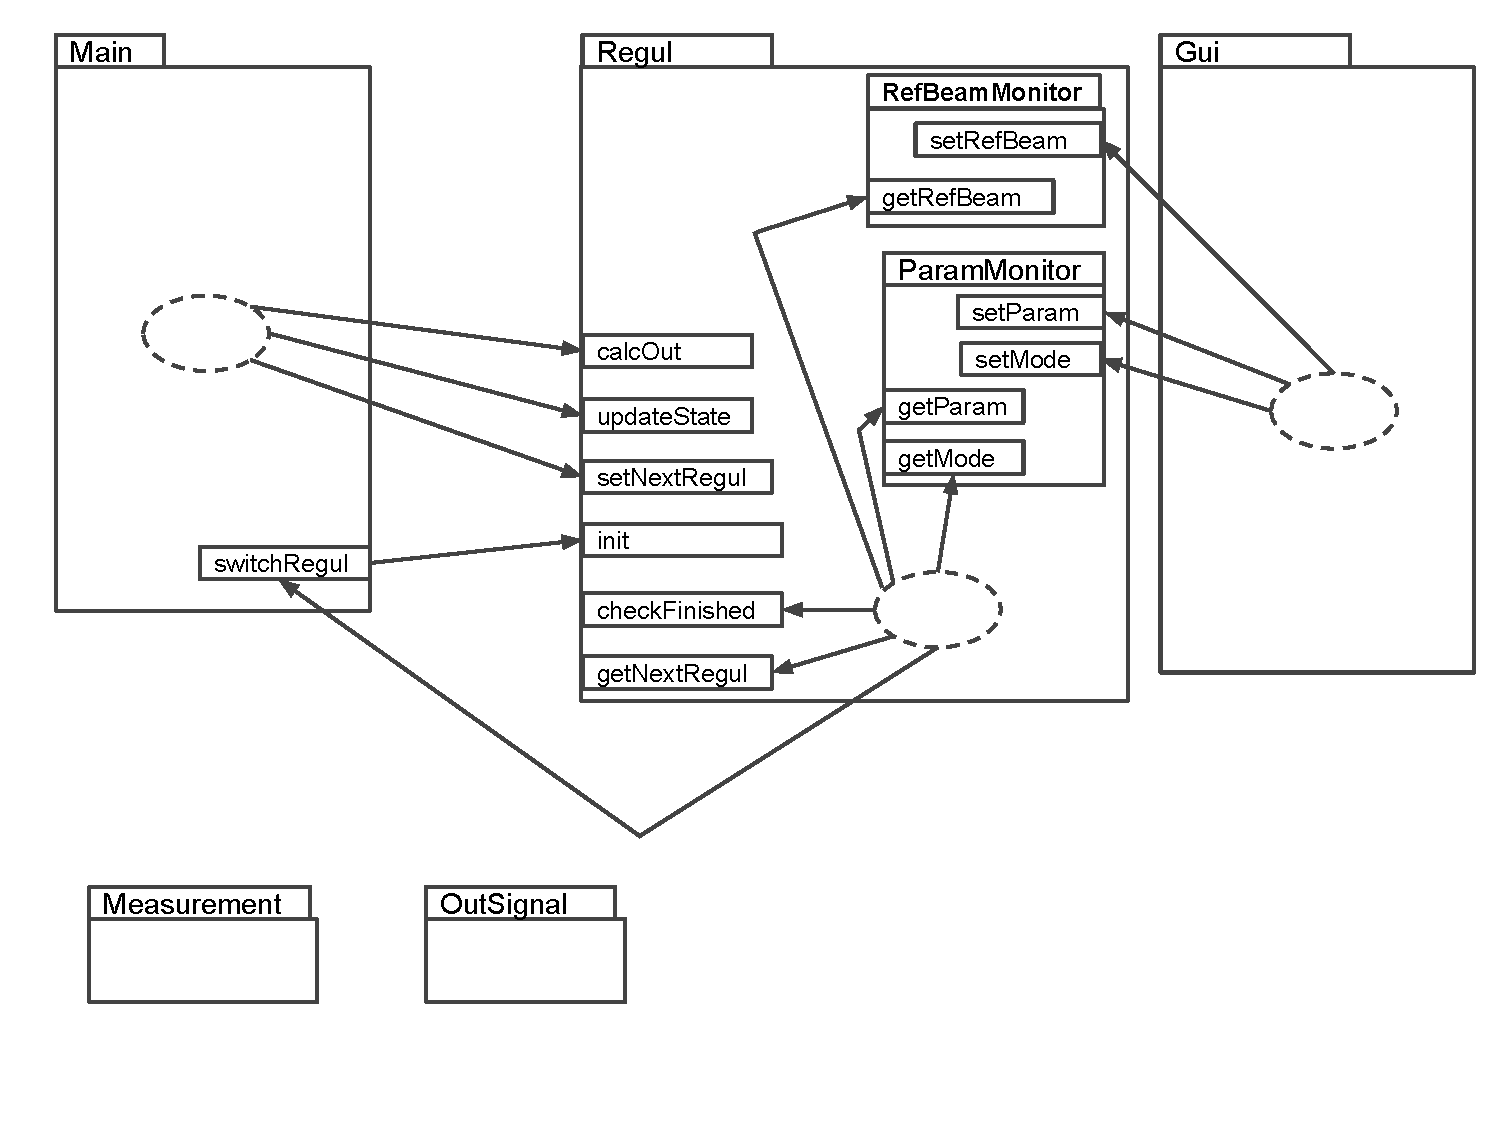
\includegraphics[width=\textwidth]{UML}
%  \caption{UML diagram}\label{fig:UML}
%\end{figure}
%
%\section{Operator communication}
%\subsection{Plotters}
%We will have the following plotters:
%\begin{itemize}
%\item Beam position (reference, measurement and Kalman filter estimate)
%\item Ball position (reference, measurement and Kalman filter estimate)
%\item Control signal
%\end{itemize}
%
%\subsection{Modes}
%We intend to implement three different modes; Beam control, Ball balancing and finally the entire sequence control scheme described in section \ref{regstruc} (beam control, ball balancing, ball delivery).
%\subsubsection{Beam control mode}
%In this mode only the beam will be controlled by a PID controller. The user should be able to tune the PID parameters as well as altering the reference value online.
%
%\subsubsection{Ball balancing mode}
%As discussed in section \ref{step2}, either LQG or cascaded PID will be used when balancing the ball for measuring its weight, and the ball balancing mode will use the same controller.
%
%If cascaded PID controllers will be used, the user will be able to tune PID parameters as well as altering the reference value for the ball. If LQG will be used however, controller parameters (weighting matrices and noise intensities) will not be as straight-forward to change online (the Riccati equations need to be resolved by some Java package or Java-\textsc{Matlab} communication). Also a reference value change would affect the linearization point, and a relinearization would be appropriate although for the same reason not very straight-forward. Therefore, with an LQG setup the controller parameters as well as reference value will only be able to change online if time permits.
%
%\subsubsection{Sequence control mode}
%In the sequence control mode, we want to test the performance of the full sequence when adjusting parameters. Therefore, a change of parameters in this mode should only affect the following iteration, and not the current one.
%
%As for the previous mode, online Riccati resolving and relinearization could be difficult to achieve. Nevertheless the user should be able to tune PID parameters as well as change the position interval for the beam when searching for the correct position to pickup a ball. If time permits, also some of the following could be allowed for an online change:
%\begin{itemize}
%\item LQG weighting matrices for ball balancing
%\item Desired ball position when estimating its weight
%\item LQG weighting matrices for ball delivery
%\item Desired final state for ball delivery
%\item LQG noise intensities (same for balancing and delivery)
%\end{itemize}
%
%\section{Timetable}
%\subsection{Workflow}
%The following tasks are equivalent to those described in section \ref{regstruc}:
%\begin{enumerate}
%	\item Get beam into position to receive ball
%	\item Weigh ball
%	\item Throw ball
%\end{enumerate}
%\subsection{Schedule}
%\begin{tabular}[h]{|l|p{10cm}|}
%\hline
%Week & Things to do \\ \hline
%45 (3-9 Nov) & *Sketch a preliminary solution of the problem and create timetable \\
% & *Code for regulation of beam (part 1) and ball \& beam (part 2) will be ready for testing individually on the real process  \\
% & *Have a precise list with all steps required for creating an LQG regulator, ie theoretical model, Riccati equation, estimation of other parameters that are needed (all the theory, basically). Write all these in the \LaTeX document to make report writing easier later \\
% & *Structure for the whole program will hopefully be ready (with potential suggestions from Karl-Erik), ie which classes and threads we will have and how they interact \\
%\hline
%46 (10-16 Nov) & *Hopefully we can now start testing on the real process, test with the regulator for beam only (part 1) and the one for beam \& ball (part 2), as well as estimation of parameters in the model (needed for stage 2) \\
% & *Parallel work: Two people can work on part 1 and two on part 2 \\
% & *GUI for the program \\
%\hline
%47 (17-23 Nov) & *Continued work on part 1 and 2 \\
% & *Start testing part 3 \\
%\hline
%48 (24-30 Nov) & *Refine part 3, Kalman filter, improvements of stuff \\
%\hline
%49 (1-7 Dec) & *Refine part 3 \\
%\hline
%50 (8-14 Dec) & *12 Dec hand in report, prepare presentation \\
%\hline
%51 (15-16 Dec) & *Demonstration and presentation 16:th of Decemeber at 15:15 and 17:15 \\
%\hline
%
%\end{tabular}

